
\paragraph{}
% why
Due to the property of the SBFEM, first order triangle element will result identical eigenvalues of one.
Under this circumstances, the displacement, nodal forces and energy using eigenvalues failed as the they are always equal to the order of the shape function, one.
As a consequence, the triangular elements shall be merged with their neighbours to form a larger polygon.
Besides, due to the fact that triangular elements are formed by cutting with the geometric boundary, triangular elements have a higher chance to be obtuse triangles, which lead to poor quality mesh.
As a result, merging triangle can help to improve the mesh quality as well.

\begin{figure}[!ht]
    \begin{subfigure}[b]{0.5\linewidth}
        \centering
        \scalebox{0.8}{
            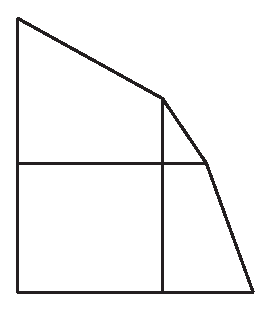
\includegraphics{adaptivity/images/adap_mt_int_before.eps}
        }
    \caption{before}
    \end{subfigure}
    \begin{subfigure}[b]{0.5\linewidth}
        \centering
        \scalebox{0.8}{
            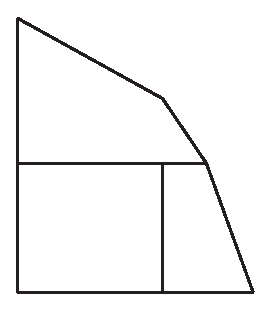
\includegraphics{adaptivity/images/adap_mt_int_after.eps}
        }
    \caption{after}
    \end{subfigure}
    \caption[Merging triangle]{Merging triangle}
    \label{adap_fig:mt_introduction}
\end{figure}

\paragraph{}
There are three steps to perform a triangle merging.
\begin{enumerate}
    \item Finding the polygon to merge with
    \item Merging triangle with the polygon
    \item Adjusting scaling center
\end{enumerate}

\paragraph{}
The first step of merging triangle is to find the appropriate cell to merge with.
Generally speaking, there will be two or three candidate as shown in fig.~\ref{adap_fig:mt_choose}
Since triangular elements are always generated by cut by the boundary, one of these possibility must contain the other part of the origin cell (cell 2 in fig.~\ref{adap_fig:mt_choose}).
However, as the cut by the boundary is necessary, undo the cut could be meaningless.
As a result, this possibility can be ignored.
If there are two remaining possibility as in fig.~\ref{adap_fig:mt_choose_3p}, the triangle will be merged with the cell that share the longer edge with it.
Triangle $0$ in fig.~\ref{adap_fig:mt_choose_3p} will be merged with cell $1$ instead of $3$ because $AB > AC$.
It is because of the following reason.
Take fig.~\ref{adap_fig:mt_choose_3p} as an example, edge $AD$ will be extended to $DC$ if triangle $0$ is merged with polygon $1$.
So merging triangle with the polygon that share a longer edge with means the polygon will less elongated and leads to a better mesh quality.
Furthermore, the polygon to merge with the triangle must have the same material property with the triangular element, otherwise they shall not be combined together.
In some extreme case, the merging triangle may not be possible as the triangular element itself fill the whole region with a specific material property.
A reasonable selection of hyperparameter in generating mesh can prevent it from happening.

\begin{figure}[!ht]    
    \begin{subfigure}[b]{0.5\linewidth}
        \centering
        \scalebox{0.8}{
            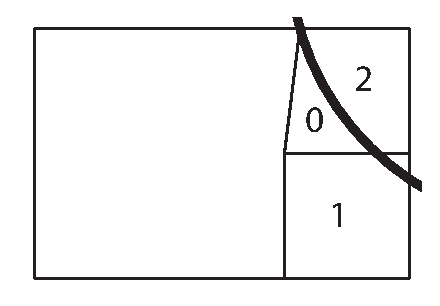
\includegraphics{adaptivity/images/adap_mt_choose_2pos}
        }
        \caption{Two possibility}
    \end{subfigure}
    \begin{subfigure}[b]{0.5\linewidth}
        \centering
        \scalebox{0.8}{
            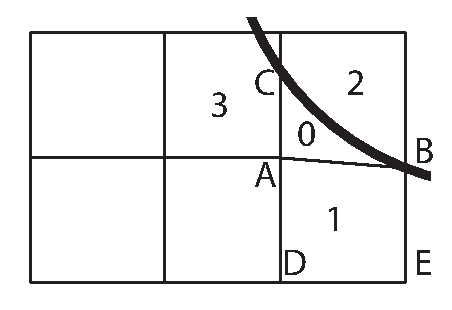
\includegraphics{adaptivity/images/adap_mt_choose_3pos}
        }
        \caption{Three possibility}
        \label{adap_fig:mt_choose_3p}
    \end{subfigure}    
    \caption[Choose the cell to merge with]{Choose the cell to merge with}
    \label{adap_fig:mt_choose}
\end{figure}

\paragraph{}
The second step which is merging the triangular element with the polygon is straightforward.
It should be noted that one point (point $A$ in fig.~\ref{adap_fig:mt_choose_3p}) is possible to be removed.
A calculation of the distance from point $A$ to line $CD$ can always help to determine whether the point can be removed or not.

\paragraph{}
% centroid
The last step is to find the scaling center for the new generated polygon.
Due to the fact that the merged polygon is very unlikely to be a polygon that looks like a square, taking the mean of all vertexes as the scaling center may not be a good idea.
Calculating the geometric center of the polygon and take it as the scaling center may be an optimized solution.
The centroid $C$ of a polygon with $n$ points $\{(x_1,y_1),(x_2,y_2),\dots,(x_n,y_n)\}$ can be calculated as
\begin{equation}
    \begin{aligned}
        C_x &= \frac{1}{6A} \sum_{i=0}^{n-1}\left(
            x_i + x_{i+1}    
        \right) \left(
            x_i y_{i+1} - x_{i+1} y_i
        \right) \\
        C_y &= \frac{1}{6A} \sum_{i=0}^{n-1}\left(
            y_i + y_{i+1}    
        \right) \left(
            x_i y_{i+1} - x_{i+1} y_i
        \right)
    \end{aligned}
\end{equation}
where $A$ stands for the area of the polygon.

\paragraph{}
% concave polygon
However, centroid of a concave polygon may be located at the outside of the polygon, result in an invalid scaling center.
Consequently, special treatment is need to adjust the scaling center.
If the mesh in the previous steps are correct, there should not be more than one reflexive angle in the polygon.
So the vertex of that reflexive angle must be found first.
It can be easily done by check the cross product between any two adjacent edges as vectors and find the only one whose sign is different with others.
An angle bisector then is drawn and the intersection between it with the edge of the polygon will be recorded (point $B$ in fig.~\ref{adap_fig:mt_concave_sc}).
The mid point of line $AB$ will be select as the scaling center of that concave polygon.

\begin{figure}[!ht]
    \centering
    \scalebox{0.8}{
        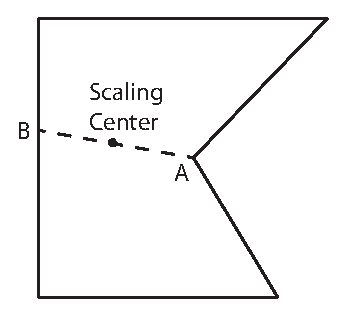
\includegraphics{adaptivity/images/adap_mt_concave_sc.eps}
    }
    \caption[Scaling center for concave polygon]{Scaling center for concave polygon}
    \label{adap_fig:mt_concave_sc}
\end{figure}

\pagebreak